\section{Teoretiske fejl}
\iffalse
\begin{frame}{Sætning 4.6}{}
    \begin{theorem}
    Let $t \geq 2$, and suppose $\mathcal{T}_h$ is a shape-regular triangulation of $\OO$. Then there exists a constant $c$ such that
    \begin{equation}
        \|u - I_h u\| _{m,h} \leq c h^{t-m} |u|_{t, H^t(\OO)}, \quad \forall u \in H^t(\OO), \quad 0 \leq m \leq t,
    \end{equation}
    where $I_h u$ denotes the interpolation by a piecewise polynomial of degreee $t-1$.
    \end{theorem}
\end{frame}
\begin{frame}{Bevis}
    \begin{equation}
        ||u-I_h u||_{m,T_j} \leq c h^{t-m} |u|_{t,T_j}, \quad \forall u \in H^t(T_j)
    \end{equation}
    \begin{align}
        \begin{split}
        ||u-I_h u||_{m,T_j} &\leq c ||B^{-1}||^m |\det B |^{1/2} |\hat{u} - I_h \hat{u}|_{m,T_{\text{ref}}} \\
                            &\leq c ||B^{-1}||^m |\det B |^{1/2} c | \hat{u} |_{t,T_{\text{ref}}} \\
                            &\leq c ||B^{-1}||^m |\det B |^{1/2} \cdot c ||B||^t \cdot |\det B |^{-1/2} |u|_{t,T}  \\
                         &\leq c {\left( ||B||  \cdot ||B^{-1}|| \right)}^m ||B||^{t-m} |u|_{t,T}.
        \end{split}
    \end{align}
\end{frame}
\begin{frame}{Bevis}
\begin{equation}
    ||B|| \leq \frac{r_2}{\rho_1}.
\end{equation}
    Shape regularity: $r_i / \rho_i \leq \kappa$ for all $T_i$ in $\mathcal{T}$

    $$||B|| \cdot ||B^{-1}|| \leq \frac{r_i \hat{r}}{\rho_i \hat{\rho}} \leq \left( 2 + \sqrt{2} \right)\kappa$$
    Og
    $$||B|| \leq h/\hat{\rho}\leq 4h$$
    \begin{equation}
        ||u-I_h u||_{m,T_j} \leq c h^{t-m} |u|_{t,T}
    \end{equation}
%VI HAR SKIFTET \ell OG m
\end{frame}
\fi
\begin{frame}{$H$-regularitet}
\begin{align*}
    \mathcal{M}^k_0 =& \{ v \in L_2(\OO) \,|\, v|_T \in \mathcal{P}_k \text{ for alle } T \in \mathcal{T}_h \} \cap C^0(\OO) \\
    =& \{ v \in L_2(\OO) \,|\, v|_T \in \mathcal{P}_k \text{ for alle } T \in \mathcal{T}_h \} \cap H^1(\OO) .
\end{align*}
    \begin{theorem}
    Suppose $\mathcal{T}_h$ is a family of shape-regular triangulation of $\Omega$. 
    Then the finite element approximation $u_h\in S_h = \mathcal{M}^k_0$, $k\geq 1$ satisfies
    \begin{align}
        \begin{split}
            \|u-u_h\|_1&\leq ch\|u\|_2\ \\
            &\leq ch\|f\|_0.
        \end{split}
        \label{eq:7.3}
    \end{align}\label{thm:7.3}
    \end{theorem}
\end{frame}

\begin{frame}{Aubin–Nitsche}
    \begin{theorem}
    Let $H$ be a Hilbert space with norm $|\cdot|$ and a scalar product $(\cdot,\cdot)$.
    Let $V\subset H$ be a Hilbert space for another norm $\|\cdot\|$, let the imbedding
    $V \hookrightarrow H$ be continuous,
    and $\forall g \in H$, let $\varphi_g \in V$ denote the unique weak solution to 
    \begin{equation}
        a(w,\varphi_g) = (g,w) \quad \forall w\in V. \label{eq:aubin_nitsche_antagelse}
    \end{equation}
    Here $a(\cdot,\cdot)$ is a bilinear continuous form.
    Then the finite element solution $u_h\in S_h \subset V$ obeys
    \begin{equation*}
        |u-u_h| \leq C \|u-u_h\| \sup_{g\in H} \left \{ \frac{1}{|g|} \inf_{v \in S_h} \|\varphi_g - v\| \right \},
    \end{equation*}
    where $\sup$ is over all $g\in H$ such that $|g|\neq 0$.
    \end{theorem}
\end{frame}

\iffalse    Vi starter med
    \begin{equation*}
        (g,w) \leq |g| \cdot |w| \implies \frac{(g,w)}{|g|} \leq |w|.
    \end{equation*}
    \begin{equation}
        \sup_{g\in H} \frac{(g,w)}{|g|} = |w|. \label{eq:duality_argument}
    \end{equation}
    \fi
\begin{frame}{Bevis}
    Undersøg finite element solution
    \begin{align*}
        a(u,v) &= f(v) \quad \forall v \in V, \\
        a(u_h,v) &= f(v) \quad \forall v \in S_h\\
        &\Downarrow \\ 
        a(u-u_h,v) &= 0 \quad \forall v \in S_h
    \end{align*}
\end{frame}
\begin{frame}{Bevis}
    \begin{align*}
        (g,u-u_h) &= a(u-u_h,\varphi _g) \\
                  &=a(u-u_h, \varphi_g -v) \\
                  &\leq C \|u-u_h\| \cdot \|\varphi_g-v\|.
    \end{align*}

    \begin{align*}
        |u-u_h| &= \sup_{g\in H} \frac{(g,u-u_h)}{|g|} \\
        &\leq C \| u-u_h\| \sup_{g\in H} \left \{ \frac{1}{|g|} \inf_{v \in S_h} \|\varphi_g - v\| \right \}.
    \end{align*}
\end{frame}

\begin{frame}{Anvendt Aubin-Nitsche}
    \begin{theorem}
   Assume $\mathcal{T}_h$ is a family of shape regular triangulations of $\OO$.
   If $u\in H^1(\OO)$ is the solution of the variational problem, then 
   \begin{equation*}
    \|u-u_h\|_0 \leq cCh \|u-u_h\|_1.
   \end{equation*}
   If $f\in L_2(\OO)$ and $u\in H^2(\OO)$, then 
   \begin{equation*}
    \|u-u_h\|_0 \leq cC^2h^2 \|f\|_0.
   \end{equation*}
    \end{theorem}
\end{frame}
\begin{frame}{Bevis}
    \begin{equation*}
        H = H^0(\OO)=L_2(\OO) \quad \text{and} \quad V = H^1_0(\OO).
    \end{equation*}

    \begin{equation*}
        |\cdot| = \|\cdot\|_0 \quad \text{and} \quad \|\cdot\| = \|\cdot\|_1,
    \end{equation*}

    \begin{equation*}
        \|u-u_h\|_0 \leq C \|u-u_h\|_1 \sup_{g\in H} \left \{ \frac{1}{|g|} \inf_{v \in S_h} \|\varphi_g - v\|_1 \right \},
    \end{equation*}
\end{frame}

\section{Numerisk Analyse}
\begin{frame}{Opstilling af problem}
\begin{equation*}
    k(x,y) = \e^{x+y}\cos(x)\sin(y)+x  \quad\text{on }\Omega
\end{equation*}
\begin{alignat*}{2}
    Lu &= -\text{div }\nabla k \quad && \text{on } \Omega \\
    u &= k \quad && \text{on } \partial \Omega,
\end{alignat*}
\end{frame}

\begin{frame}{Domæne}
\begin{figure}
    \centering
    \begin{subfigure}{.49\textwidth}
        \centering
        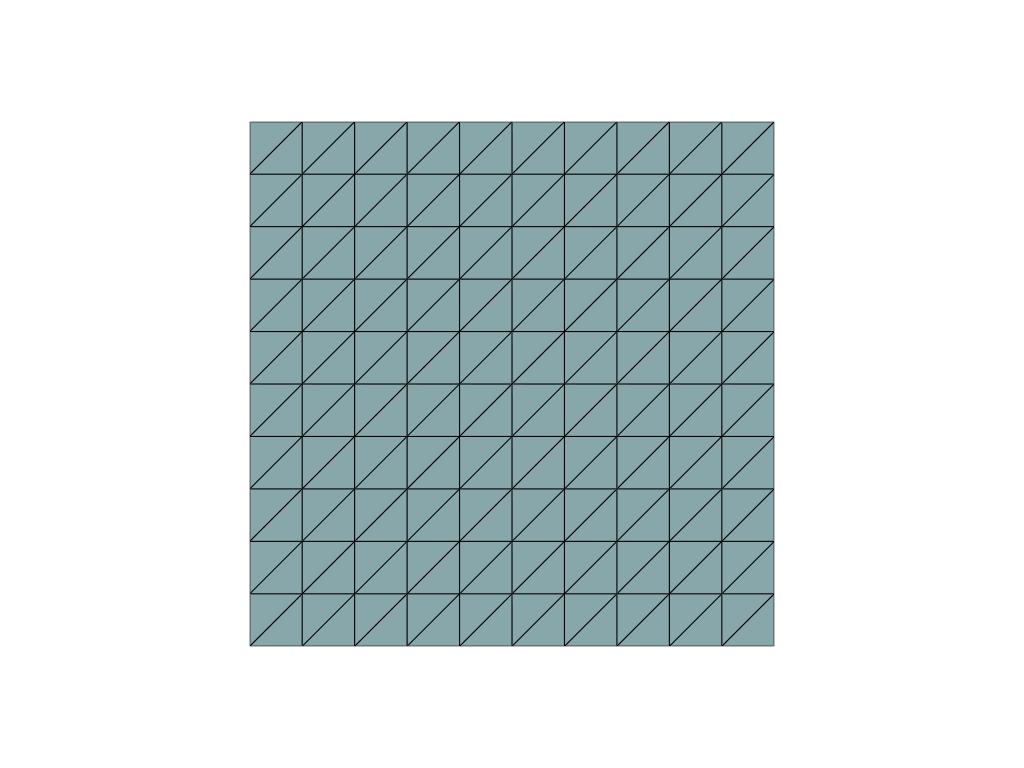
\includegraphics[width=\textwidth]{figurer/screenshot_1.jpeg}
      \end{subfigure}
    \begin{subfigure}{.49\textwidth}
        \centering
        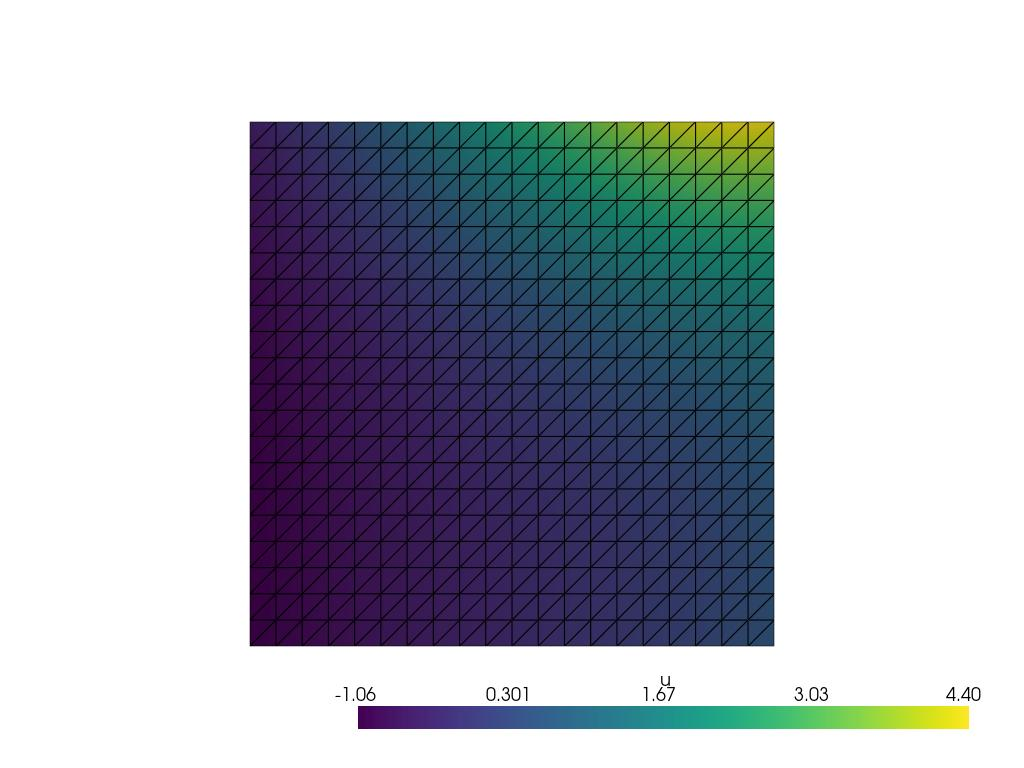
\includegraphics[width=\textwidth]{figurer/screenshot_2.jpeg}
    \end{subfigure}
    \begin{subfigure}{.49\textwidth}
        \centering
        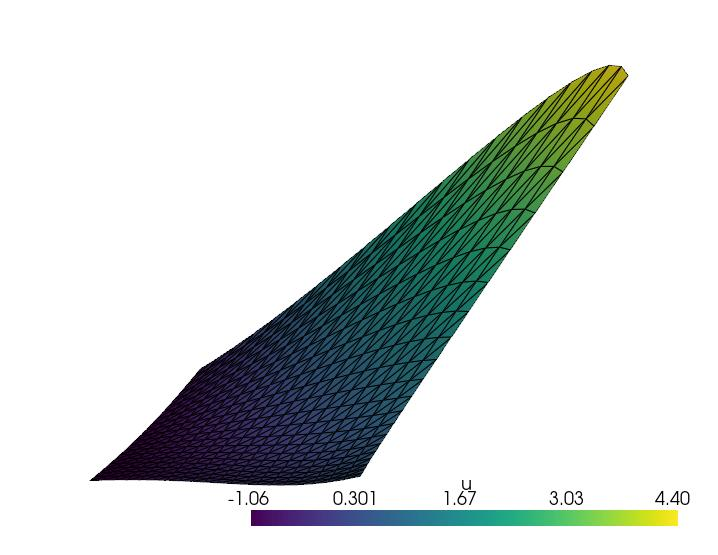
\includegraphics[width=\textwidth]{figurer/screenshot_3.jpeg}
    \end{subfigure}
\end{figure}
\end{frame}
\subsection{Plot af fejl}
\begin{frame}{Brug af $L_2$}
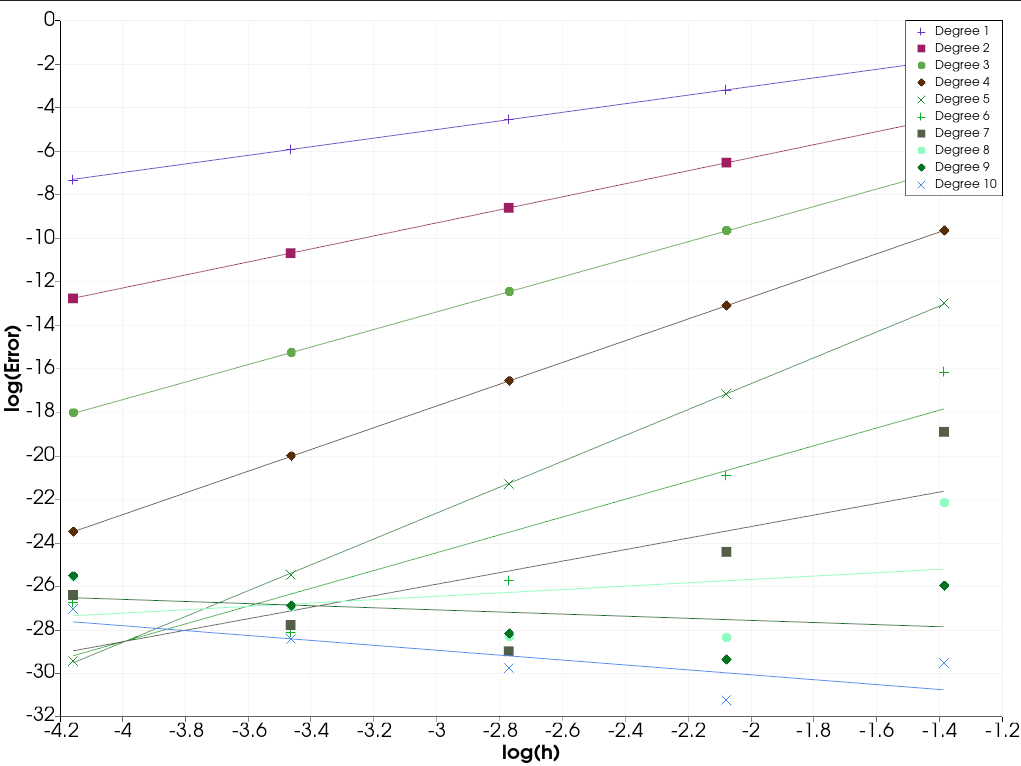
\includegraphics[width=\textwidth]{figurer/l2-fejl-plot.jpeg}    
\end{frame}
\begin{frame}{Brug af $H^1$}
   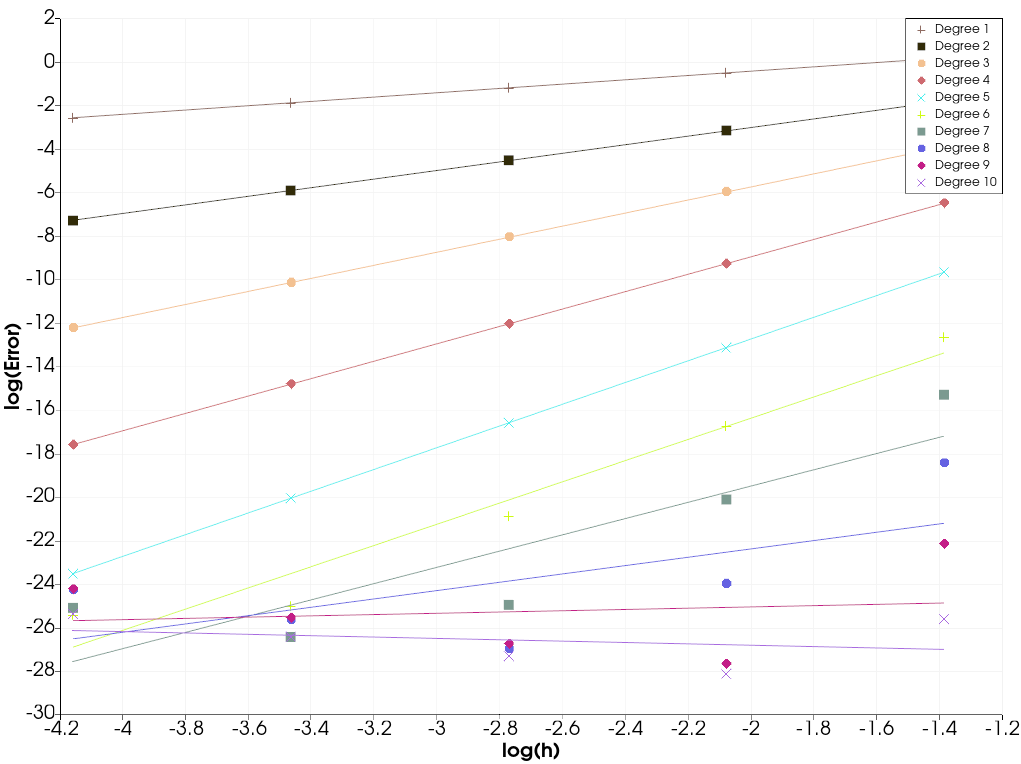
\includegraphics[width=\textwidth]{figurer/h1-fejl_plot.png} 
\end{frame}